\section{Понятие растра и связности. Растеризация и её этапы. Сглаживание. Растровое представление отрезка. Алгоритм Брезенхейма.}
\begin{center}
    Конспект составил: \textit{Рафик Нурмухаметов}
\end{center}

\subsection{Основные понятия}
\subsubsection*{Растр}
Растр в компьютерной графике~--- это способ представления изображения в виде двумерной сетки, состоящей из пикселей. Пиксель в данном случае является минимальной неделимой единицей изображения, который характеризуется положением и цветом.

Растровые изображения имеют фиксированное разрешение, которое определяется количеством пикселей по ширине и высоте. Чем выше разрешение, тем более детализированное изображение получается, но также увеличивается объем памяти, необходимый для хранения и обработки.
\subsubsection*{Связность}
Связность~--- это свойство растра, которое определяет, какие пиксели в растре считаются соседними. Это понятие критически важно для алгоритмов обработки изображений. Существуют два основных подхода:
\begin{itemize}
    \item 4-связность: пиксель считается соседним только с теми пикселями, которые примыкают по горизонтали или вертикали (на рисунке 1 представлены серыми точками).
    \item 8-связность: помимо горизонтальных и вертикальных соседей, также учитываются пиксели, примыкающие по диагонали (на рисунке 1 представлены белыми точками).
\end{itemize}

\begin{figure}[H]
    \centering
    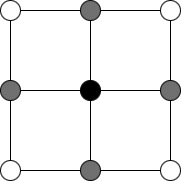
\includegraphics[width = 4cm]{cohesion.jpg}
    \caption{4- и 8-связность.}
    \label{fig:float}
\end{figure}
Выбор вида связности зависит от алгоритма обработки и специфики задачи.

\subsubsection*{Понятие растеризации и её этапы}
Чтобы перейти от непрерывного пространства точек $P_1(x, y)$ к дискретному $P_2(\tilde{x}, \tilde{y})$, необходимо выполнить растеризацию~--- процесс, который позволяет каждой точке из исходного непрерывного пространства найти свое соответствие в двумерной сетке.

\paragraph*{Определение ячейки}
Для точки $(x, y)$ необходимо определить, в какую ячейку она попадает. Для этого можно использовать целочисленное деление. Разделим каждую координату на соответствующий размер ячейки ($\Delta x$ - размер ячейки по горизонтали, $\Delta y$ - по вертикали), отбросив дробную часть (это действие переведет координаты в индекс ячейки на сетке), а затем домножим на этот же размер ячейки (чтобы вернуться в физическое пространство):
\[
    x^* = (x \ \texttt{//} \ \Delta x) * \Delta x
\]
\[
    y^* = (y \ \texttt{//} \ \Delta y) * \Delta y
\]
На рисунке 2 проиллюстрировано, что происходит с точкой $(6, 9)$ на заданной сетке после данных манипуляций.
\begin{figure}[H]
    \centering
    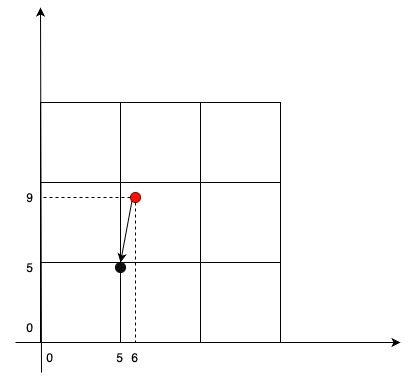
\includegraphics[width = 5cm]{second_step.jpg}
    \caption{Процесс определения ячейки.}
    \label{fig:float}
\end{figure}

\paragraph*{Определение угла ячейки}
После определения того, в какой ячейке лежит точка $(x, y)$, необходимо определить, к какому из углов она ближе. Для этого определим для каждой координаты необходимость смещения следующим образом:
\[
    b_x = ((x - x^*) * 2 \geq \Delta x)
\]
\[
    b_y = ((y - y^*) * 2 \geq \Delta y)
\]
Будем считать что $b_x$ и $b_y$ равны единице, если соответствующие равенства выполняются и нулю в противном случае. Конечный результат будет выглядеть следующим образом:
\[
    \tilde{x} = x^* + b_x * \Delta x
\]
\[
    \tilde{y} = y^* + b_y * \Delta y
\]
На рисунке 3 проиллюстрировано, что происходит с точкой после данных манипуляций.
\begin{figure}[H]
    \centering
    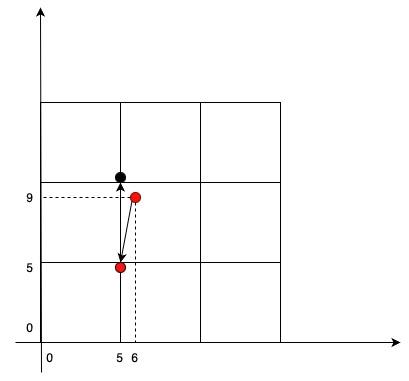
\includegraphics[width = 5cm]{third_step.jpg}
    \caption{Процесс определения угла.}
    \label{fig:float}
\end{figure}

\subsubsection*{Сглаживание}
Сглаживание~--- это метод уменьшения визуальных искажений, возникающих в процессе растеризации, таких как «лесенки», которые наиболее часто появляются при прорисовке наклонных или криволинейных объектов. Цель сглаживания заключается в том, чтобы сделать границы объектов более плавными и естественными.

\paragraph*{Одна точка}
Для сглаживания цвет распределяется не только на центральный пиксель, но и на его соседей. Это позволяет добиться эффекта плавного перехода между цветами. Пример распределения интенсивности цвета для одного пикселя:
\begin{itemize}
    \item Центральный пиксель получает основную часть интенсивности (например, 100\% или FF в шестнадцатеричной системе).
    \item Горизонтальные и вертикальные соседи получают меньшую часть интенсивности (например, 50\% или FF/2).
    \item Диагональные соседи получают ещё меньшую интенсивность (например, 25\% или FF/4, либо 12.5\% или FF/8).
\end{itemize}

\begin{figure}[H]
    \centering
    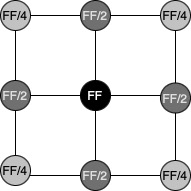
\includegraphics[width=5cm]{smooth_one.jpg}
    \caption{Пример сглаживания (одна точка).}
    \label{fig:float}
\end{figure}

\paragraph*{Две точки}
Когда нужно подсветить две точки, находящиеся рядом, их области влияния на пиксели начинают пересекаться. В этом случае интенсивности цветов объединяются (например, можем взять максимальную интенсивность), что делает переход между точками ещё более плавным.

\begin{figure}[H]
    \centering
    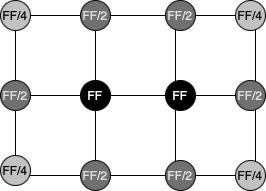
\includegraphics[width=6cm]{smooth_two.jpg}
    \caption{Пример сглаживания (две точки).}
    \label{fig:float}
\end{figure}

\subsubsection*{Растровое представление отрезка}
Пусть имеется прямая, проходящая через точки $(x_1, y_1)$ и $(x_2, y_2)$. Ставиться следующая задача~--- определить, какие точки двумерного растра нужно закрасить, чтобы получить достаточно близкое приближение данной прямой между закрашенными точками.

Не умаляя общности, будем считать, что наша прямая ``идёт'' вправо вверх. Зная точки, через которые проходит прямая, можем описать уравнение, задающее данную прямую: $y = y_1 + x * \frac {y_2 - y_1} {x_2 - x_1}$. Идея заключается в том, что мы начинаем идти по всем точкам $\tilde{x_1} + \Delta x, \ \tilde{x_1} + 2\Delta x, \ ..., \tilde{x_1} + n \Delta x = \tilde{x_2}$, считая при этом и округляя с точностью до $\Delta x$ значение $f(\tilde{x_i} + i *\Delta x)$. Здесь $\Delta x$ - размер ячеек по горизонтали.

\begin{figure}[H]
    \centering
    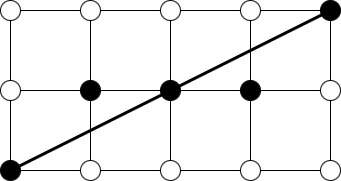
\includegraphics[width = 7cm]{basic_line.jpg}
    \caption{Растровое представление отрезка.}
    \label{fig:float}
\end{figure}

Основная проблема данного подхода~--- использование ``дорогостоящей'' арифметики с плавающей точкой и постоянные округления.

\paragraph*{Алгоритм Брезенхэма}
Алгоритм Брезенхэма~--- алгоритм, позволяющий определить, какие точки двумерного растра нужно закрасить, для того, чтобы получить наиболее близкое приближение прямой линии между двумя заданными точками. Идея алгоритма Брезенхэма заключается в том, чтобы на каждом шаге выбирать пиксель, который минимизирует ошибку отклонения от идеальной прямой, при этом частично или полностью исключая вычисления с плавающей точкой.

\begin{figure}[H]
    \centering
    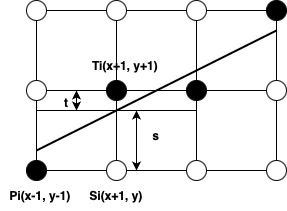
\includegraphics[width = 7cm]{brezenhein_line.jpg}
    \caption{Растровое представление отрезка с помощью алгоритма Брезенхема.}
    \label{fig:float}
\end{figure}

Рассмотрим отрезок на рисунке 2, который соединяет некоторые точки, допустим, $(x_1, y_1)$ и $(x_2, y_2)$. Обозначим $\Delta x = x_2 - x_1$ и $\Delta y = y_2 - y_1$ и предположим, что $\Delta x \geq 0$ и $\Delta y \geq 0$.

Пусть первая точка находится ближе к началу координат. Тогда вычтем из соответствующих координат каждой точки $x_1$ и $y_1$, перенеся таким образом первую точку в начало координат, а вторую в $(\Delta x, \Delta y)$.

Зная точки, через которые проходит прямая, мы можем задать её через уравнение $y = y_1 + x * \frac {y_2 - y_1} {x_2 - x_1}$. С учетом вышесказанного, уравнение примет вид $y = x \frac{\Delta y}{\Delta x}$. Из рисунка 7, ввиду подобия треугольников, следует, что
\[
    \frac{\Delta y}{\Delta x} = \frac{s + y}{x + 1} \Rightarrow s = \frac{\Delta y}{\Delta x} * (x + 1) - y
\]
\[
    t = y + 1 - \frac{\Delta y}{\Delta x} * (x + 1),
\]
откуда получаем
\[
    s - t = 2 \frac{\Delta y}{\Delta x}*(x+1) - 2y - 1.
\]
Домножим обе части равенства на $\Delta x$
\[
    \Delta x (s - t) = 2(\Delta y * x - y * \Delta x) + 2 \Delta y - \Delta x.
\]
Так как $\Delta x \geq 0$, то можем использовать величину $ \Delta x (s-t) $ в качестве критерия для выбора пикселя. Обозначим данную величину через $d_i:$
\[
    d_i = 2(\Delta y * x_{i-1} - y_{i-1} * \Delta x) + 2 \Delta y - \Delta x.
\]
\[
    d_{i+1} = 2(\Delta y * x_{i} - y_{i} * \Delta x) + 2 \Delta y - \Delta x.
\]
Так как величу $d_i$ надо считать на каждом шаге, рассчитаем приращение $d_{i+1} - d_{i}$, которое обозначим как $\Delta_i$:
\[
    \Delta_i = d_{i+1} - d_i = 2 \Delta y (x_i - x_{i-1}) - 2 \Delta x(y_i - y_{i-1}).
\]
Известно, что $x_i - x_{i-1} = 1$.

Если величина $d_i \geq 0$, тогда выбираем $T_i$, то есть $y_i - y_{i-1} = 1$ (перемещаем точку по $y$), а приращение $\Delta_i = 2 (\Delta y - \Delta x)$.

Если величина $d_i < 0$, тогда выбираем $S_i$, то есть $y_i - y_{i-1} = 0$ (значение $y$ не меняется), а приращение $\Delta_i = 2 \Delta y$.

Начальное значение будет иметь вид $d_1 = 2\Delta y - \Delta x$. Таким образом, мы получили итеративную формулу для вычисления критерия $d_i$ (часто вместо ``критерий'' можно услышать ``ошибка'').

Следует отметить, что данный алгоритм требует дополнительного параметра~--- значения, определяющего изменение $y_i$. В примере мы предположили, что $\Delta y \geq 0$, и, соответственно, при перемещении точки значение увеличивалось на 1. Если же $\Delta y < 0$, то изменение происходит на -1.
Аналогично рассматривается случай, когда $\Delta x < \Delta y$.
